In this first lecture, we see why randomness and quantum computation matter for two basic problems,
primality/factoring and search. We introduce random sampling as the basic primitive of randomized
algorithms, prove a lower bound of $n-1$ queries for deterministic search, and review the basics of
probability that we need for the rest of the course.

\section{Efficient Algorithms and Finding Prime Numbers}

Consider the problem of deciding whether a given number $n$ is prime. The input is the binary
representation of $n$, so the \emph{input size} is the number of bits $N = \log_2 n$.

\begin{definition}[Efficient Algorithm]
    An algorithm is \textbf{efficient} if it runs in time polynomial in the input size, i.e., in time
    $\bigO{N^k}$ for some constant $k$. For primality testing this means time
    $\bigO{(\log_2 n)^k}$.
\end{definition}

Trial division by all numbers up to $\sqrt{n}$ takes $\bigTh{\sqrt{n}} = \bigTh{2^{N/2}}$ time,
which is exponential in the input size. A deterministic polynomial-time algorithm exists
(time $\tilde{\mathcal{O}}(N^{12})$, later improved to $\tilde{\mathcal{O}}(N^{6})$),
but it is not used in practice.

\subsection{Randomized Algorithms}

The algorithm used in practice is \emph{randomized}. The Miller--Rabin test decides primality with
high probability in $\bigO{N^3}$ time. If $n$ is composite, then at least
$\sfrac{3}{4}$ of the numbers in $\set{2, \dots, n-2}$ are \emph{witnesses} of the fact that $n$ is
composite, while a prime has no witness. So after $k$ independent samples a composite $n$ goes
undetected with probability at most $\left(\sfrac{1}{4}\right)^k$: the answer ``composite'' is always
right, and the answer ``prime'' is wrong with probability at most $\left(\sfrac{1}{4}\right)^k$.

\section{Random Sampling}

All that a randomized algorithm needs is the ability to \emph{sample}. We assume that flipping a
(fair) coin is an $\bigO{1}$ time primitive.

\subsection{Sampling a Random Element of an Array}

Consider an array with $n$ slots (\cref{fig:coinflips-0825}), $n$ a power of $2$. Every index is a
bit string of $\log_2 n = \log n$ bits, so flipping one coin for each bit samples a uniformly random
element in $\bigO{\log n}$ time:
$\prob{\text{index $i$ is chosen}} = \left(\sfrac{1}{2}\right)^{\log n} = \sfrac{1}{n}$ for every $i$.

\begin{figure}[ht]
    \centering
    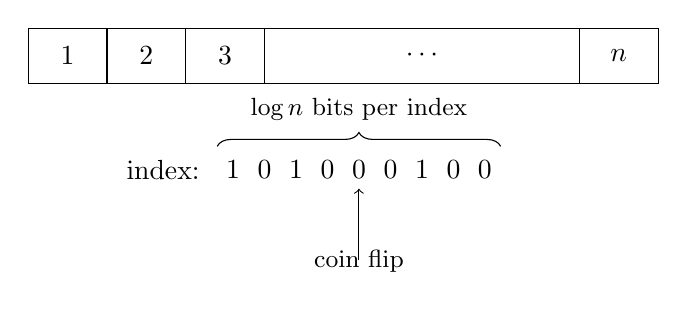
\begin{tikzpicture}
        % the array
        \draw (0,0) rectangle (8,0.7);
        \foreach \x in {1,2,3,7} {\draw (\x,0) -- (\x,0.7);}
        \node at (0.5,0.35) {$1$};
        \node at (1.5,0.35) {$2$};
        \node at (2.5,0.35) {$3$};
        \node at (5,0.35) {$\cdots$};
        \node at (7.5,0.35) {$n$};
        % an index, written as a bit string
        \node[anchor=east] at (2.3,-1.1) {index:};
        \foreach \x/\b in {0/1,1/0,2/1,3/0,4/0,5/0,6/1,7/0,8/0} {
                \node (b\x) at (2.6+0.4*\x,-1.1) {$\b$};
            }
        \draw[->] (b4.south) ++(0,-0.9) -- (b4.south);
        \node[below] at (4.2,-2.0) {\small coin flip};
        \draw[decorate, decoration={brace, amplitude=5pt}] (2.4,-0.8) -- (6.0,-0.8)
        node[midway, above=6pt] {\small $\log n$ bits per index};
    \end{tikzpicture}
    \caption{Each of the $\log n$ bits of the index is one coin flip.}
    \label{fig:coinflips-0825}
\end{figure}

We usually assume that an element can be sampled in constant time. This is only justified when the
space we sample from has polynomial size in $n$, since then the number of coin flips is
$\bigO{\log n}$.

\subsection{With and Without Replacement}

Random sampling can be done \emph{with} or \emph{without} replacement. We almost always analyze
sampling with replacement, since without replacement the samples are no longer independent.

Suppose that we are looking for one particular element of the array. Every sample hits it with
probability $\sfrac{1}{n}$, so sampling (with replacement) until it is found takes
$\expectation{\text{samples}} = \frac{1}{\sfrac{1}{n}} = n$ samples in expectation, and since the
samples are independent,
\[\prob{\text{not found after $k$ samples}} = \left(1 - \frac{1}{n}\right)^k,
    \qquad
    \prob{\text{found within $k$ samples}} = 1 - \left(1 - \frac{1}{n}\right)^k.\]

\section{Factoring}

Given $n = pq$ with $p, q$ prime, find $p$ and $q$. Factoring is an \emph{encryption primitive}: if
it can be solved quickly, then encryption based on it is broken. No polynomial-time (in
$N = \log n$) classical algorithm is known, but \emph{Shor's factoring algorithm} is a quantum
algorithm that runs in polynomial time $\bigO{N^3}$. There is \emph{no} known quantum algorithm that
solves \nptime-complete problems in polynomial time.

Recall that \nptime{} is the class of problems whose solutions can be verified in polynomial time,
and that the \nptime-complete problems are the \nptime{} problems to which every \nptime{} problem
reduces (equivalently, the problems that are reducible to 3-SAT and vice versa). Whether
$\textsc{P} = \nptime$ is open. A quantum computer can simulate a classical one with polynomial
overhead, so if quantum computers cannot solve \nptime-complete problems in polynomial time, then
$\textsc{P} \neq \nptime$.

\section{Search}

We are given an (unsorted) array $A$ with $n$ slots, which can only be accessed through
\emph{queries} (``what is $A[i]$?''), and we want to find the index of a given element $x$. A
sorted array allows binary search with $\bigO{\log n}$ queries. Linear search makes $\bigO{n}$
queries.

\subsection{Lower Bound for Deterministic Algorithms}

An upper bound needs one algorithm, but a lower bound of $\bigOm{f(n)}$ has to hold for \emph{all}
algorithms. We use an \emph{adversary argument}: given any algorithm, the adversary constructs an
input on which the algorithm performs badly.

\begin{theorem}[Lower Bound for Deterministic Search]\label{thm:detsearch-0825}
    Every deterministic algorithm for search makes at least $n - 1$ queries in the worst case.
\end{theorem}

\begin{proof}
    Fix a deterministic algorithm. The adversary does not fix the input in advance: whenever the
    algorithm queries a slot $i$, it answers that $A[i] \neq x$ (and fills $A[i]$ with some other
    value). Since the algorithm is deterministic, its $\nth{k}$ query is determined by the answers
    to the first $k-1$ queries, so this defines one run of the algorithm. Suppose that it stops
    after $k \leq n - 2$ queries and outputs an index $j$. At least $n - k \geq 2$ slots have not
    been queried, so the adversary can place $x$ in an unqueried slot different from $j$. The
    resulting array is consistent with all the answers given, and the algorithm is wrong on it. So a correct
    algorithm makes at least $n - 1$ queries.
\end{proof}

\subsection{Randomized and Quantum Algorithms}

The adversary argument breaks down for \emph{randomized} algorithms, because the queries are no
longer determined by the previous answers. Still, randomized search needs $\bigOm{n}$ expected
queries, by \emph{Yao's min-max principle} (next lecture). Grover's quantum algorithm solves search
with $\bigO{\sqrt{n}}$ queries (later in the course).

To show a \emph{quantum advantage} (also called quantum supremacy) for a problem, we have to
show that it needs $\bigOm{f(n)}$ queries classically but only $\littleO{f(n)}$ queries
quantumly.

\section{Probability}

A \textbf{sample space} $S$ is a finite set of \emph{simple events}, $\abs{S} = n$. A
\textbf{probability function} $\Pr \colon S \to [0,1] \subseteq \mathbb{R}$ assigns a probability to every
simple event. An \textbf{event} is a subset $A \subseteq S$, with probability
$\prob{A} = \sum_{a \in A} \prob{a}$. The probability function satisfies the \emph{axioms}
$\prob{A} \geq 0$ for every event $A$, $\prob{S} = 1$, and
$\prob{A_1 \cup A_2 \cup \dots \cup A_n} = \sum_{i=1}^{n} \prob{A_i}$ for pairwise disjoint events
$A_1, \dots, A_n$ (i.e., $A_i \cap A_j = \emptyset$ for all $i \neq j$). A \textbf{random variable} is a
function $X \colon S \to V$ from the sample space to a set of values $V$ (usually $V \subseteq \mathbb{R}$),
and for a value $r \in V$, $\prob{X = r} = \sum_{s \in S \,:\, X(s) = r} \prob{s}$.
